\section{Herstellung des Rohres}
Für diesen Versuch wurde in einem CAD-Programm das Modell eines Pitotrohres erstellt und dieses in einem 3D-Drucker gedruckt. Nach einigen Versuchen haben wir es so geschafft, ein funktionsfähiges Pitot-Rohr herzustellen.

\section{Messung der Fahrgeschwindigkeiten}
Um die Geschwindigkeiten des fahrenden Autos zu messen, wurde das Pitotrohr am Dach des Autos befestigt (Siehe Abbildung \ref{rohre}), zusammen mit einer schon vorrätigen Prandtlsonde, welche zur Messung des statischen Druckes verwendet wurde. Diese sind mit einem Feinmanometer im Inneren des Autos verbunden worden. Mit einer ersten Kamera wurde der Stand des Manometers sowie parallel die von einem GPS-Sensor ausgegebene Geschwindigkeit aufgenommen (Siehe Abbildung \ref{messung}), mit einer zweiten die Anzeige des Tachometers. Die beiden Aufnahmen wurden über die Audiospur synchronisiert, um die drei Geschwindigkeiten zu jeweils einem bestimmten Zeitpunkt auswerten zu können.

\begin{figure}
\centering
	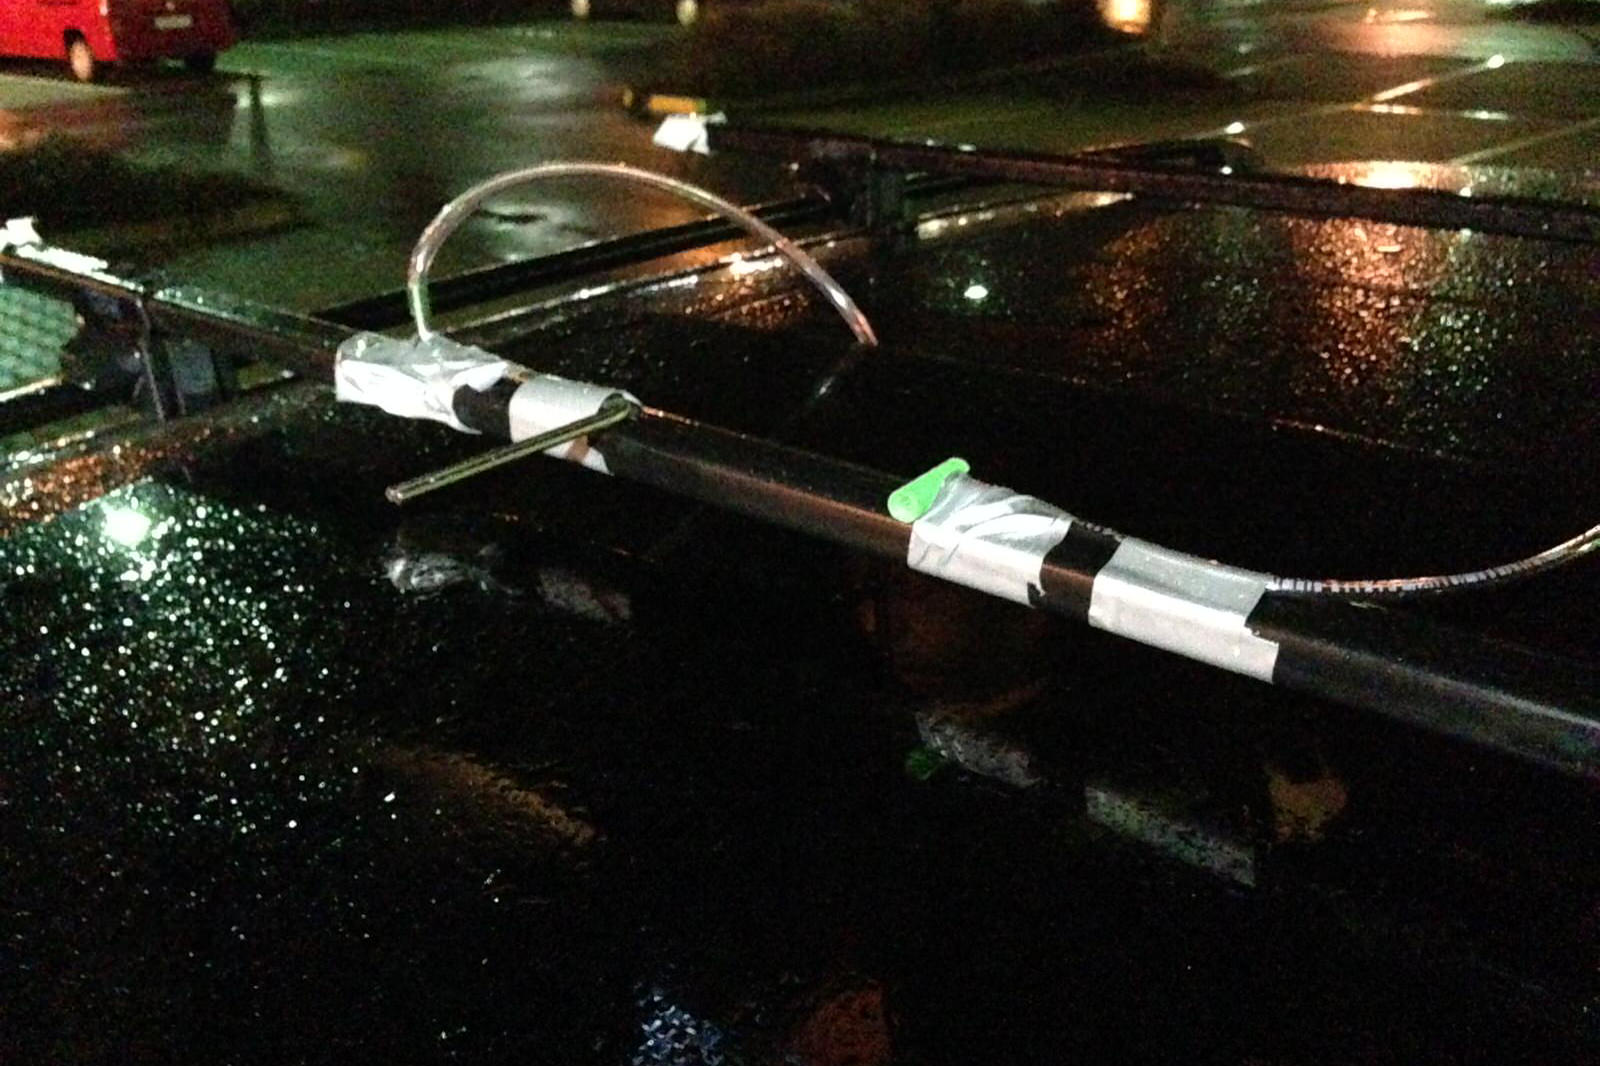
\includegraphics[width=.8\textwidth]{images/rohre.jpg}
	\caption{Bild des Versuchsaufbaus auf dem Autodach}
	\label{rohre}
\end{figure}

\begin{figure}
\centering
	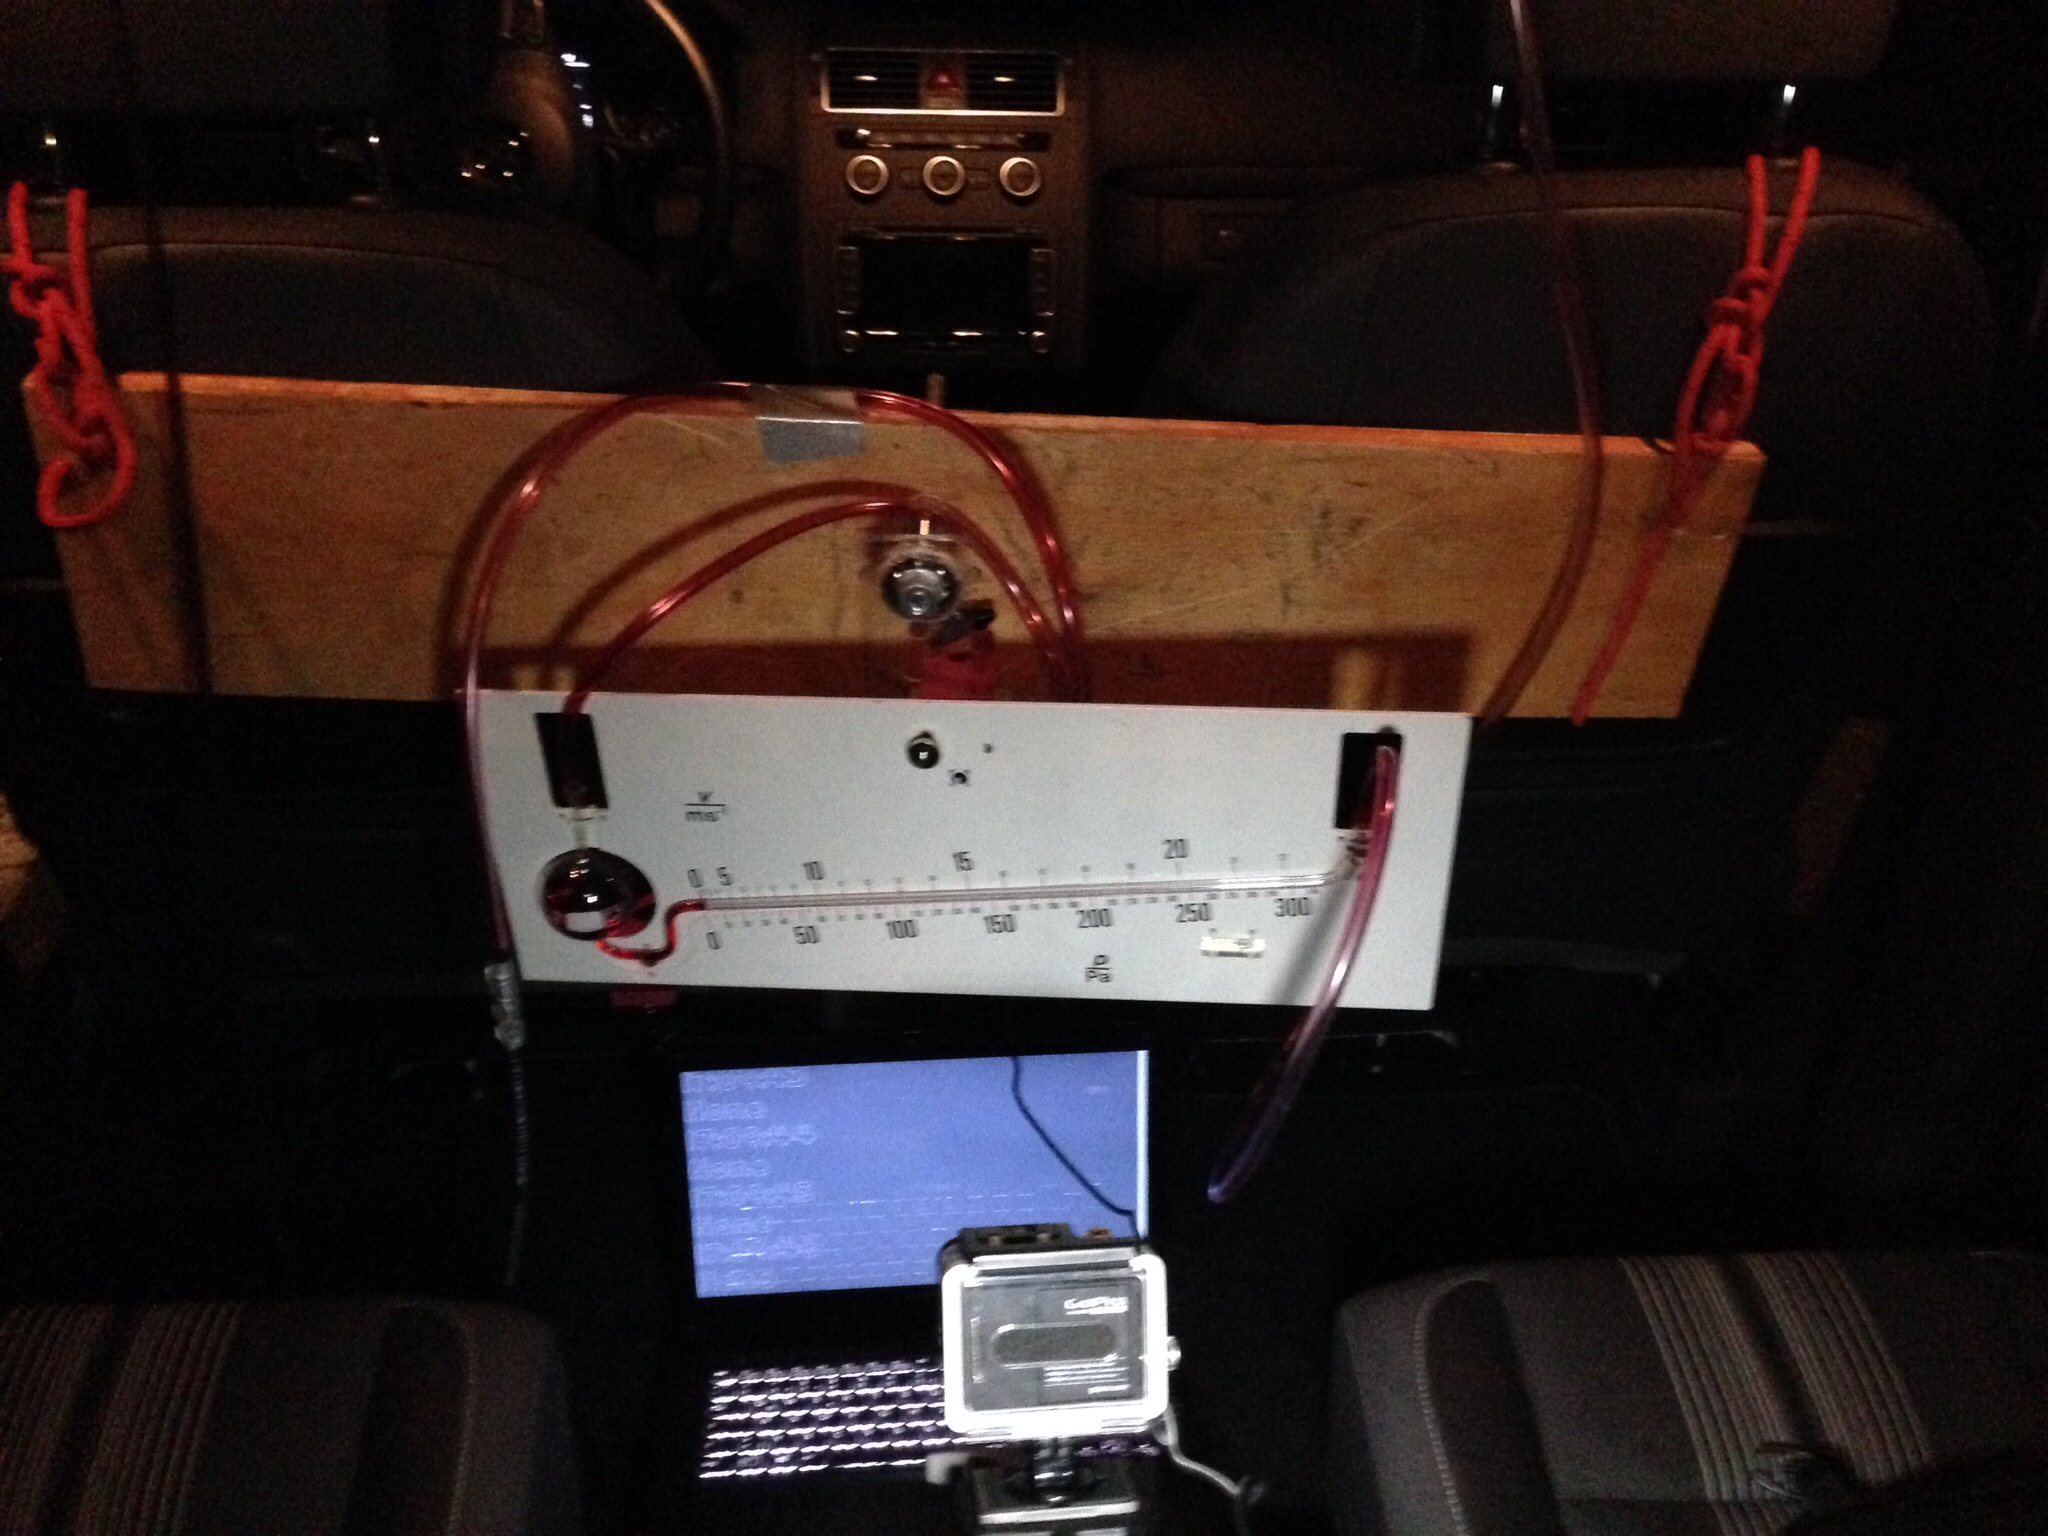
\includegraphics[width=.8\textwidth]{images/messung.jpg}
	\caption{Feinmanometer und Laptop mit GPS-Sensor}
	\label{messung}
\end{figure}

\subsection{Aufhängung des Feinmanometers}
Um mit dem Feinmanometer messen zu können, muss es genau senkrecht zur Beschleunigung ausgerichtet werden. Dies wurde im Auto mittels einer kardanischen Aufhängung realisiert (Siehe Abbildung \ref{aufhängung}): in eine frei im Auto, parallel zur Windschutzscheibe hängende Holzplatte wurde das Manometer mittels eines Kugellagers an einer Gewindestange befestigt und diese in ein Loch in der Mitte der Holzplatte eingelassen. Dies garantiert die waagrechte Ausrichtung des Manometers im Auto und gleicht leichtere Erschütterungen aus. 


\begin{figure}
\centering
	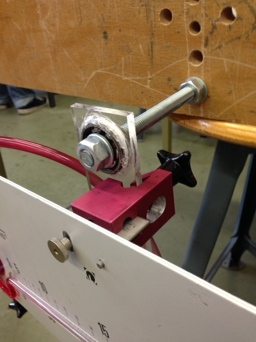
\includegraphics[width=.5\textwidth]{images/aufhaengung.JPG}
	\caption{Aufhänung des Feinmanometers}
	\label{aufhängung}
\end{figure}